%%%%%%%%%%%%%%%%%%%%%%%%%%%%%%%%%%%%%%%%%%%%%%%%%%%%%%%%%%%%%%%%%%%%%%%%%%%%%%%%%%%%%%%%%%%%%%%%
%
% CS484 Written Question Template
%
% Acknowledgements:
% The original code is written by Prof. James Tompkin (james_tompkin@brown.edu).
% The second version is revised by Prof. Min H. Kim (minhkim@kaist.ac.kr).
%
% This is a LaTeX document. LaTeX is a markup language for producing 
% documents. Your task is to fill out this document, then to compile 
% it into a PDF document. 
%
% 
% TO COMPILE:
% > pdflatex thisfile.tex
%
% If you do not have LaTeX and need a LaTeX distribution:
% - Personal laptops (all common OS): www.latex-project.org/get/
% - We recommend latex compiler miktex (https://miktex.org/) for windows,
%   macTex (http://www.tug.org/mactex/) for macOS users.
%   And TeXstudio(http://www.texstudio.org/) for latex editor.
%   You should install both compiler and editor for editing latex.
%   The another option is Overleaf (https://www.overleaf.com/) which is 
%   an online latex editor.
%
% If you need help with LaTeX, please come to office hours. 
% Or, there is plenty of help online:
% https://en.wikibooks.org/wiki/LaTeX
%
% Good luck!
% Min and the CS484 staff
%
%%%%%%%%%%%%%%%%%%%%%%%%%%%%%%%%%%%%%%%%%%%%%%%%%%%%%%%%%%%%%%%%%%%%%%%%%%%%%%%%%%%%%%%%%%%%%%%%
%
% How to include two graphics on the same line:
% 
% \includegraphics[width=0.49\linewidth]{yourgraphic1.png}
% \includegraphics[width=0.49\linewidth]{yourgraphic2.png}
%
% How to include equations:
%
% \begin{equation}
% y = mx+c
% \end{equation}
% 
%%%%%%%%%%%%%%%%%%%%%%%%%%%%%%%%%%%%%%%%%%%%%%%%%%%%%%%%%%%%%%%%%%%%%%%%%%%%%%%%%%%%%%%%%%%%%%%%

\documentclass[11pt]{article}

\usepackage[english]{babel}
\usepackage[utf8]{inputenc}
\usepackage[colorlinks = true,
linkcolor = blue,
urlcolor  = blue]{hyperref}
\usepackage[a4paper,margin=1.5in]{geometry}
\usepackage{stackengine,graphicx}
\usepackage{fancyhdr}
\setlength{\headheight}{15pt}
\usepackage{microtype}
\usepackage{times}

% From https://ctan.org/pkg/matlab-prettifier
\usepackage[numbered,framed]{matlab-prettifier}

\frenchspacing
\setlength{\parindent}{0cm} % Default is 15pt.
\setlength{\parskip}{0.3cm plus1mm minus1mm}

\pagestyle{fancy}
\fancyhf{}
\lhead{Homework 2 Questions}
\rhead{CS484}
\rfoot{\thepage}

\date{}

\title{\vspace{-1cm}Homework 2 Questions}


\begin{document}
	\maketitle
	\vspace{-3cm}
	\thispagestyle{fancy}
	
	\section*{Instructions}
	\begin{itemize}
		\item 4 questions.
		\item Write code where appropriate.
		\item Feel free to include images or equations.
		\item Please make this document anonymous.
		\item \textbf{Please use only the space provided and keep the page breaks.} Please do not make new pages, nor remove pages. The document is a template to help grading.
		\item If you really need extra space, please use new pages at the end of the document and refer us to it in your answers.
	\end{itemize}

	\section*{Questions}
	
	\paragraph{Q1:} Explicitly describe image convolution: the input, the transformation, and the output. Why is it useful for computer vision?
	
	%%%%%%%%%%%%%%%%%%%%%%%%%%%%%%%%%%%
	\paragraph{A1:} Assuming the input is $n\times n$ data and transformation is $2k+1\times 2k+1$, then the output will be $n-2k\times n-2k$ data.
	
	And convolution means
	\begin{LARGE} $$h[m,n] = \sum_{k,l} f[k,l]I[m-k,n-l]$$ \end{LARGE}
	
	%%%%%%%%%%%%%%%%%%%%%%%%%%%%%%%%%%%
	
	% Please leave the pagebreak
	\pagebreak
	\paragraph{Q2:} What is the difference between convolution and correlation? Construct a scenario which produces a different output between both operations.
	
	\emph{Please use \href{https://www.mathworks.com/help/images/ref/imfilter.html}{$imfilter$} to experiment! Look at the `options' parameter in MATLAB Help to learn how to switch the underlying operation from correlation to convolution.}
	
	%%%%%%%%%%%%%%%%%%%%%%%%%%%%%%%%%%%
	\paragraph{A2:} The most different point is the direction of the calculation. In other words, in the image, the direction in which the filter operates is different.

	2D convolution is $$h[m,n] = \sum_{k,l} f[k,l]I[m-k,n-l].$$
	2D correlation is  $$h[m,n] = \sum_{k,l} f[k,l]I[m+k,n+l].$$

	The order of the calculations is different only because the k,l sign is negative or positive.

\begin{figure}[h]
    \centering
    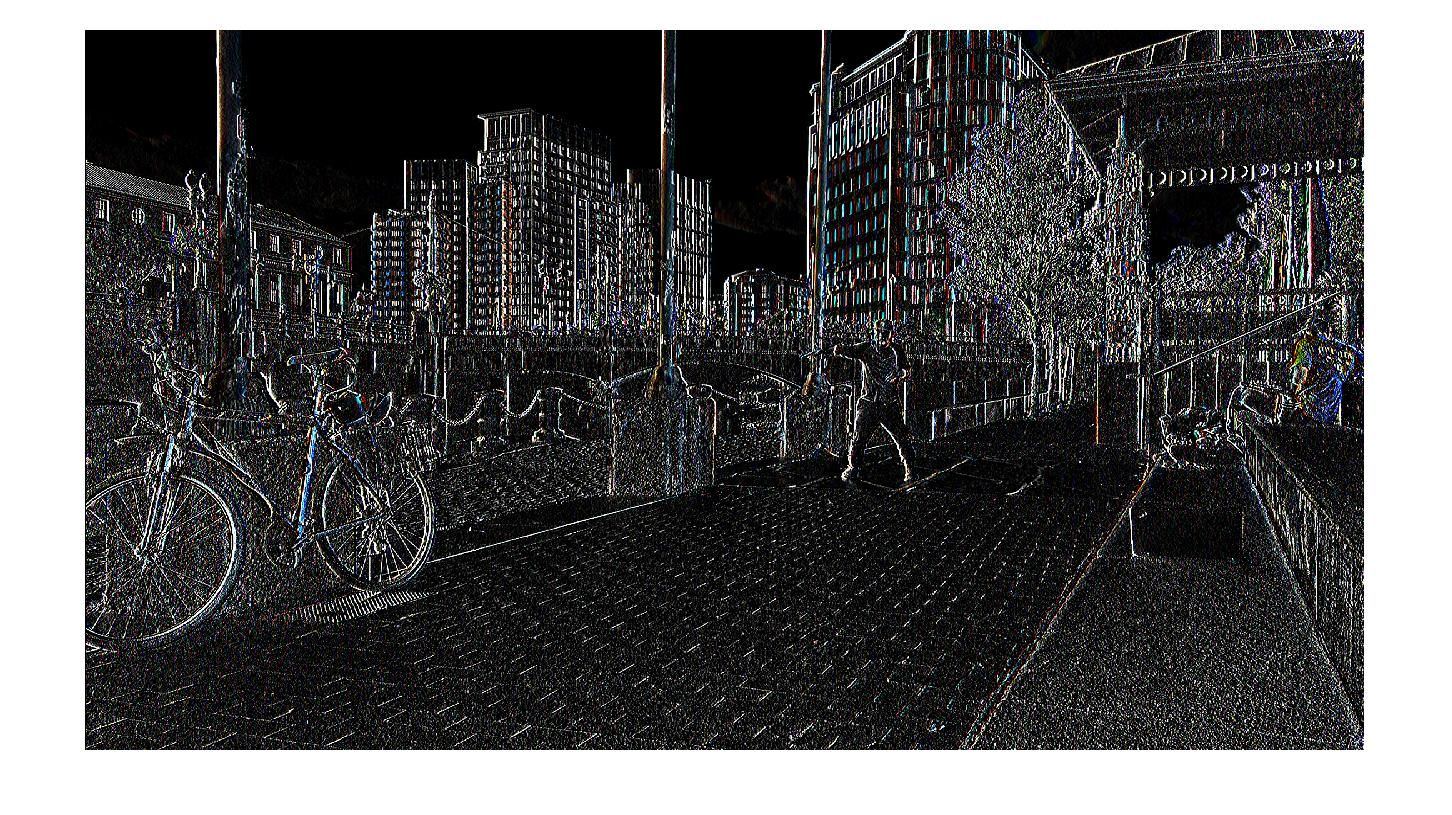
\includegraphics[width=11cm]{hw2_q2_corr.jpg}
    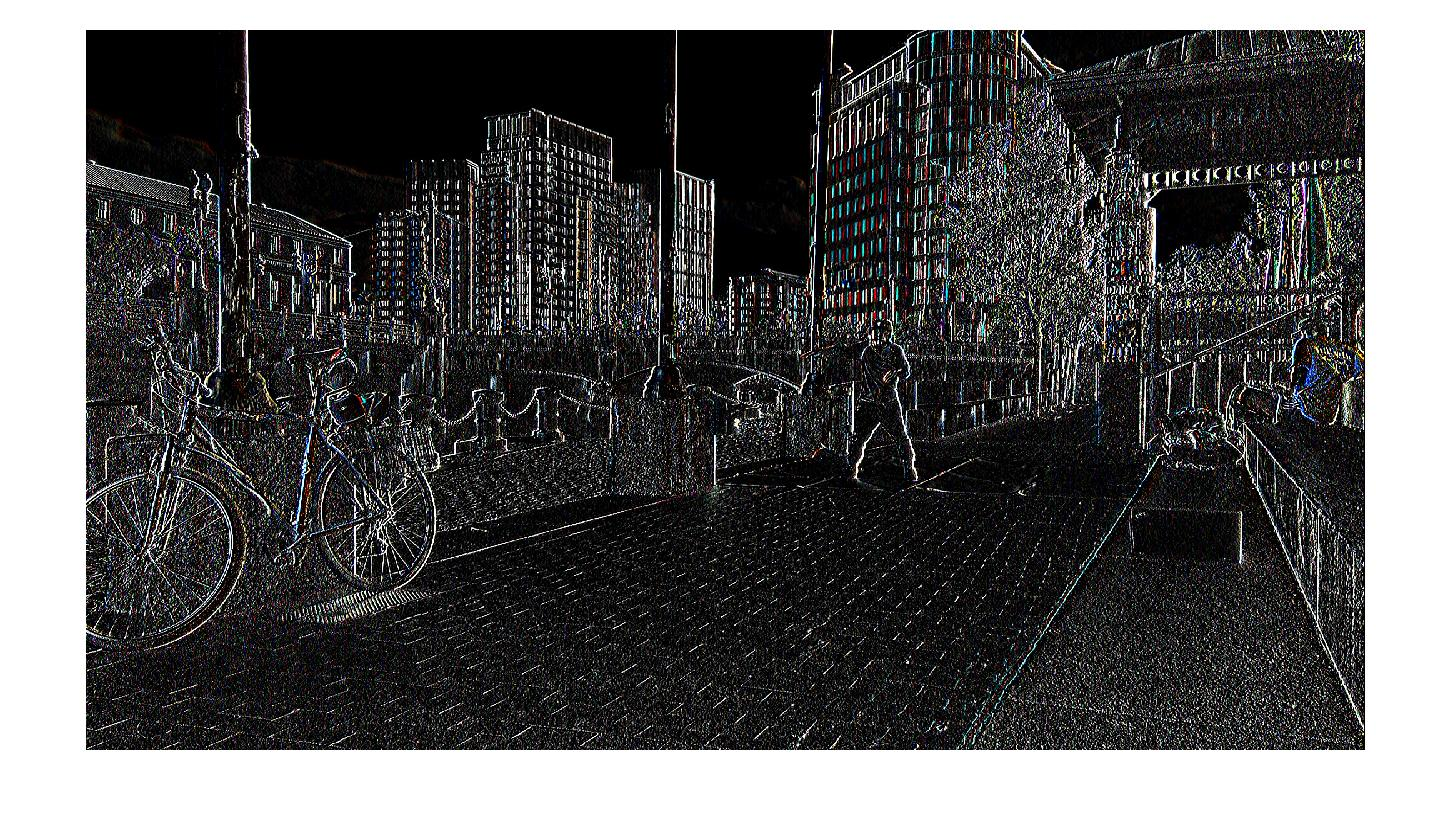
\includegraphics[width=11cm]{hw2_q2_conv.jpg}
    \caption{\emph{Up:} correlation. \emph{Down:} convolution. both use Vertical Edge(Sobel) filter.}
    \label{fig:result1}
\end{figure}

	The two pictures emphasize the opposite side of each other.
	
	
	%%%%%%%%%%%%%%%%%%%%%%%%%%%%%%%%%%%
	
	% Please leave the pagebreak
	\pagebreak
	\paragraph{Q3:} What is the difference between a high pass filter and a low pass filter in how they are constructed, and what they do to the image? Please provide example kernels and output images.
	
	%%%%%%%%%%%%%%%%%%%%%%%%%%%%%%%%%%%
	\paragraph{A3:} Your answer here.
	The low pass filter was used fspecial('gaussian',a,b) and the high pass filter was used to subtract the value of fspecial ('gaussian',a,b) from the original image. The a,b value on both sides were adjusted by viewing the picture being printed.	
There are hybrid images.
\begin{figure}[h]
	    		\centering
	    		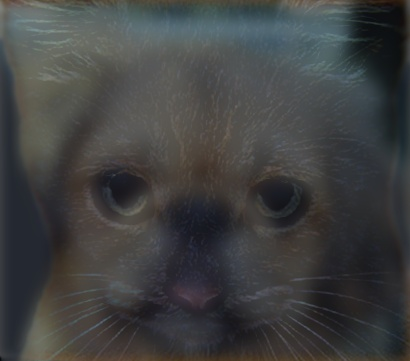
\includegraphics[width=4cm]{cat&dog.jpg}
		   	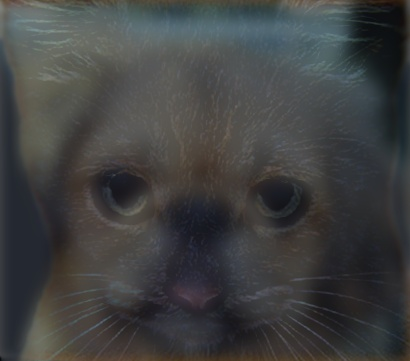
\includegraphics[width=1cm]{cat&dog.jpg}
			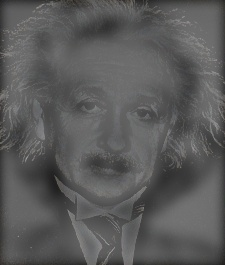
\includegraphics[width=4cm]{einstein&marilyn.jpg}
	    		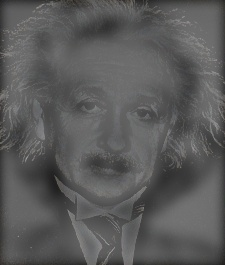
\includegraphics[width=1cm]{einstein&marilyn.jpg}
	    		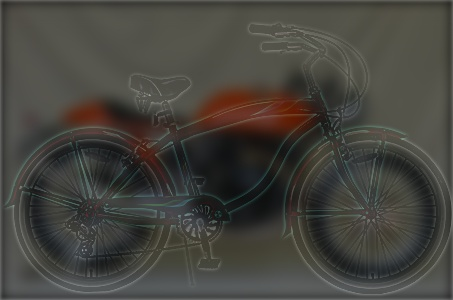
\includegraphics[width=4cm]{bicycle&motorcycle.jpg}
	    		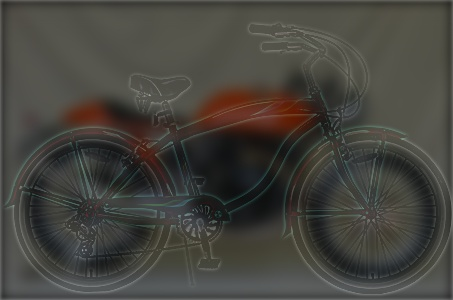
\includegraphics[width=1cm]{bicycle&motorcycle.jpg}
    			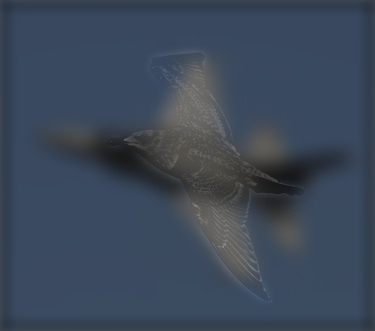
\includegraphics[width=4cm]{bird&plane.jpg}
	    		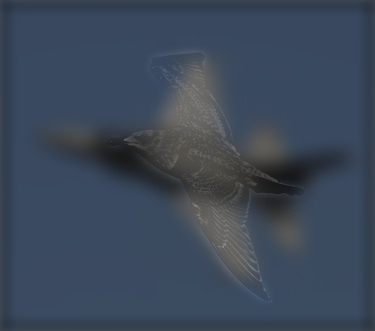
\includegraphics[width=1cm]{bird&plane.jpg}
	    		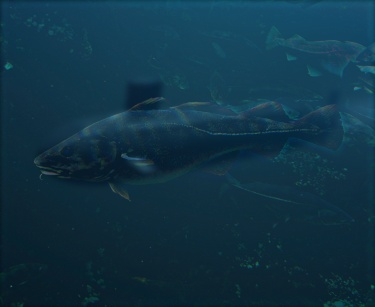
\includegraphics[width=5cm]{fish&submarine.jpg}
	    		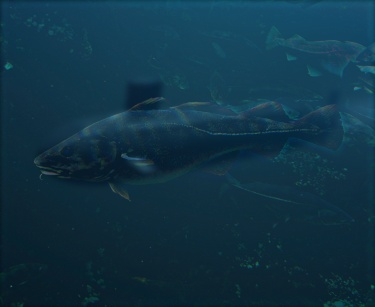
\includegraphics[width=1cm]{fish&submarine.jpg}
	    		\caption{\emph{Left:} We can see cat/einstein/bicycle/bird/fish. \emph{Right:} We can see dog/marilyn/motorcycle/palne/submarine.}
	    		\label{fig:result2}
		\end{figure}
	%

	%
	
	%%%%%%%%%%%%%%%%%%%%%%%%%%%%%%%%%%%
	
	% Please leave the pagebreak
	\pagebreak
	\paragraph{Q4:} How does computation time vary with filter sizes from $3\times3$ to $15\times15$ (for all odd and square sizes), and with image sizes from 0.25~MPix to 8~MPix (choose your own intervals)? Measure both using \href{https://www.mathworks.com/help/images/ref/imfilter.html}{$imfilter$} to produce a matrix of values. Use the \href{https://www.mathworks.com/help/images/ref/imresize.html}{$imresize$} function to vary the size of an image. Use an appropriate charting function to plot your matrix of results, such as \href{https://www.mathworks.com/help/matlab/ref/scatter3.html}{$scatter3$} or \href{https://www.mathworks.com/help/matlab/ref/surf.html}{$surf$}.
	
	Do the results match your expectation given the number of multiply and add operations in convolution?
	
	See RISDance.jpg in the attached file.
	
	%%%%%%%%%%%%%%%%%%%%%%%%%%%%%%%%%%%
	\paragraph{A4:} Your answer here.

	1. Multiple and add as large as filter size for each pixel.\\
	2. Repeat for each pixel.\\
	When the filter size is $(2k+1) \times (2k+1)$ and the number of pixels b, the total number of operations is $(2k+1) \times (2k+1) \times b \times (multiple+add)$.
	
	And the test results and codes are below.

	\begin{figure}[h]
    \centering
    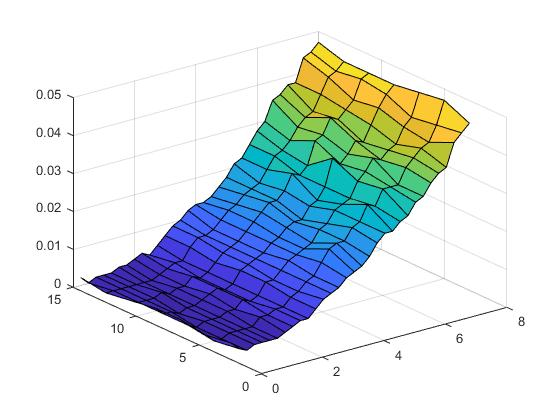
\includegraphics[width=6.5cm]{hw2_q4_graph1.jpg}
    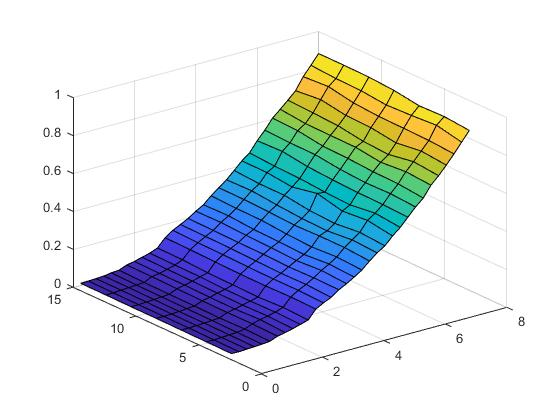
\includegraphics[width=6.5cm]{hw2_q4_graph3_20try.jpg}
    \caption{\emph{Left:} just one try. \emph{Right:} sum of 20 tries.}
    \label{fig:result3}
\end{figure}


	
	
	
	%%%%%%%%%%%%%%%%%%%%%%%%%%%%%%%%%%%
	
	
	% If you really need extra space, uncomment here and use extra pages after the last question.
	% Please refer here in your original answer. Thanks!
	%\pagebreak
	%\paragraph{AX.X Continued:} Your answer continued here.
	\pagebreak
	\paragraph{A4 Countinued:}
\begin{lstlisting}[style=Matlab-editor]
i1=im2double(imread('RISDance.jpg'));
[s1,s2,s3] = size(i1);
size1 = s1*s2*s3; 
sizegap = 262144/size1; 
Time = zeros(7,32); 
x=3:2:15; 
y=0.25:0.25:8; 
[X,Y]=meshgrid(y,x);
for a=1:7
    filter = fspecial('Gaussian', [2*a+1 2*a+1], 10);
    for b=1:32
        I = imresize(i1,sizegap*b,'bilinear');
        t1 = clock;
        for c = 1:20
            newone = imfilter(I,filter,'conv');
        end
        t2 = clock;
        Time(a,b) = etime(t2,t1);
    end
end
surf(X,Y,Time);
\end{lstlisting}
	
	
\end{document}